\section{LLM-Based Linked Text Generation}

\subsection{Introduction and Definitions}

Large Language Models (LLMs) can do several tasks, due to the large amount of data on they are trained. In the paper \textit{Language Models are Few-Shot Learners} (Brawn et al. 2020), the authors presented three different ways to improve the results of LLMs in specific tasks, without doing any \textit{fine-tuning}. We refer to these techniques as \textit{prompting strategies}. Before describing the three different prompting strategies, it is important to give some definitions.

\textbf{Definition 1: Example}. In the context of LLM, an \textit{Example} $E$ is a pair $(Q, A)$ where $Q$ is an object which contains the input for the LLM; $A$ is an object with contains the answer generated by the LLM.

\begin{figure}[!h]
    \centering
    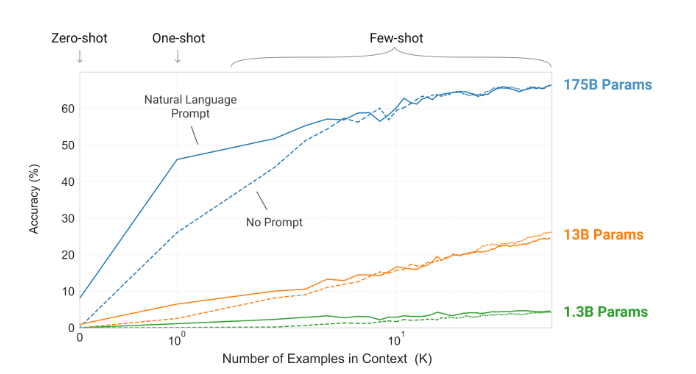
\includegraphics[width=1\linewidth]{fig/image.png}
    \caption{Larger models make increasingly efficient use of in-context information [from Brown paper]}
    \label{fig:enter-label}
\end{figure}

\textbf{Definition 2: Prompt}. In the context of LLM, a \textit{Prompt} $P$ is a pair $(C, E*)$ where $C$ represents the \textit{context} description for the task that the LLM has to perform, while $E*$ represents a list of Examples (zero or more examples).

The \textit{context} in the prompt is important, because it describes the task in which the LLM is involved, through a description that is in Natural Language (NL).

Figure \ref{fig:enter-label} highliths that the significance of $C$, in given $P$ prompt, decrease when $|E*|$ increases. Given \( E^* \) (a set), a list of prompts, and \( C \) (a context) and \textit{Relevance} a function which measure the impact of a text in the accuracy:

\[
|E^*| \to \infty \implies \text{Relevance}(C) \to 0.
\]

\subsection{Informal Design}

In this section, a description of the workflow we will implement is given. The goal of the system is mainly to generate parts of a Fluid program. In particular, starting from a textual input, like a caption, we want to replace in the caption the parts that could be generated by Fluid functions.

\begin{table*}[!ht]
    \centering
    \caption{Examples}
    \begin{tabular}{p{13cm}}
    \hline
    \hline
    \\\textbf{Input}:\\
    The SSP1-2.6 scenario caps an increase to $v1$ by the century's end, with an exceedance being unlikely. Contrastingly, SSP2-4.5 considers it likely.\\\\
    \hline
    \\\textbf{Output}:\\
    "The ", sspone.scenario, " scenario caps an increase to ", numToStr sspone.bestE81100, " by the century's end, with an exceedance being ", likelihoodMap(findLikelihood(sspone.low81100, sspone.high81100) 2.0), ". Contrastingly, ", ssptwo.scenario, " considers it ", likelihoodMap(findLikelihood(ssptwo.low81100, ssptwo.high81100) 2.0), "."\\
    \hline
    \hline
    \end{tabular}
\end{table*}

To achieve the results described above, we designed the following system architecture. Figure \ref{fig:fluid-llm-architecture} illustrates the proposed architecture.
The process begins with the input object being passed to the Recognition Agent, which analyzes the input, identifies elements to be replaced, and substitutes them with tags. The tagged content is then forwarded to the FluidGenerator Agent, which replaces the tags with the corresponding functions.
The output from this process is sent, along with the input, to the Validation phase. During this phase, the Replacing Validator ensures that changes were made exclusively to the tags. Additionally, the Parser Agent executes the generated code to validate the results.
If either validation step fails, the errors are returned to the FluidGenerator Agent for iterative correction and refinement.

\begin{figure}
    \centering
    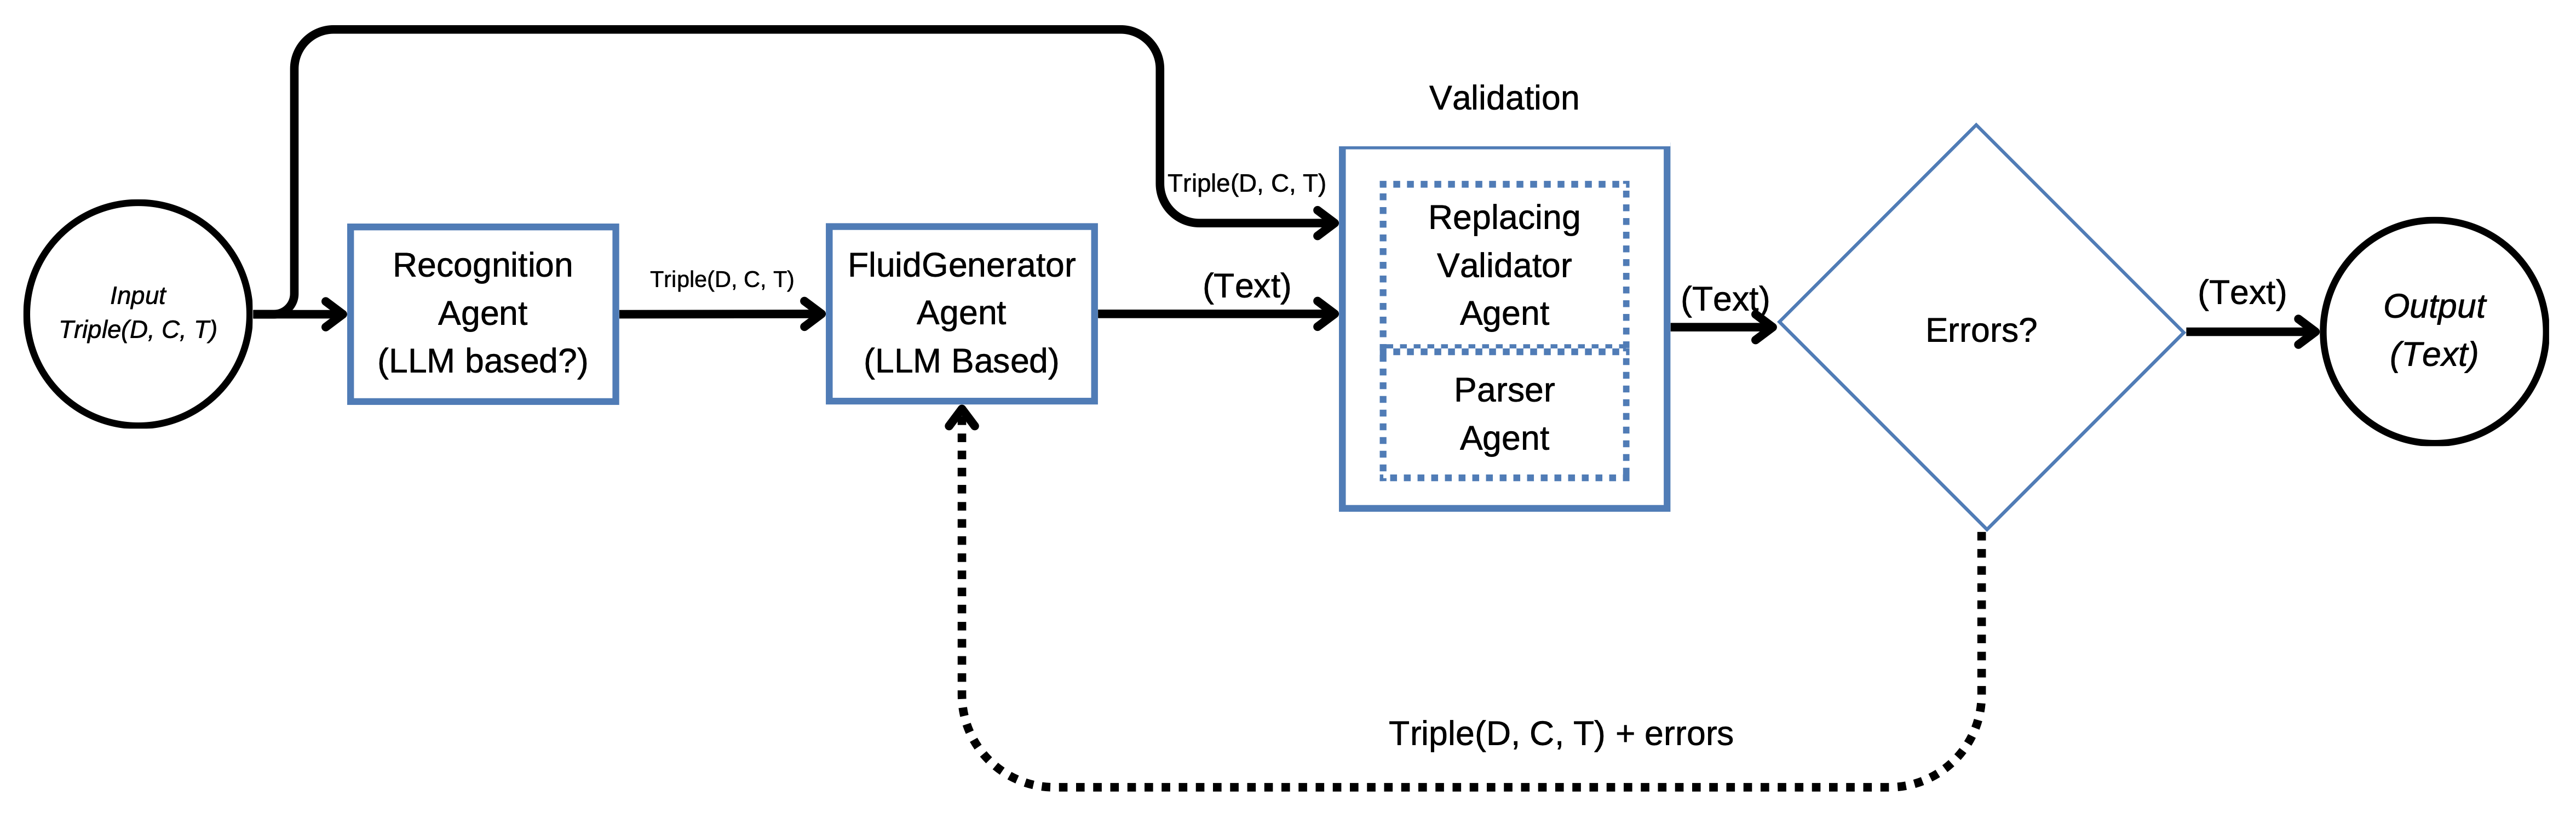
\includegraphics[width=0.95\linewidth]{fig/fluid-llm-architecture.png}
    \caption{Draft architecture of the LLM-based code generation}
    \label{fig:fluid-llm-architecture}
\end{figure}

\subsubsection{QueryContext}
The input for this system needs to describe the following information:
\begin{itemize}
    \item \textbf{Datasets}: the datasets that the fluid program is using in it. These datasets are files that have a JSON-like format.
    \item \textbf{Imports}: the fluid libraries that the program needs for working. The imports is modelled as a list of path.
    \item \textbf{Fluid Code}: The fluid program, used to link the variables to the text.
    \item \textbf{Text}: text element that the system will work on, replacing informations that can be extracted from variables or functions with the relate fluid elements.
\end{itemize}

\begin{table*}[!ht]
    \centering
    \caption{Input JSON Example \label{tab:json_fluid_input}}
    \begin{tabular}{p{13cm}}
    \hline
    \hline
    \begin{verbatim}
{
    "data": "[
    { scenario: "SSP3-7.0", bestEst2140: 1.5, low2140: 1.2, high2140: 1.7, bestEst4160:
    1.6, low4160: 1.2, high4160: 2.0, bestEst81100: 1.4, low81100: 1.0, high81100: 1.8},
    { scenario: "SSP1-1.9", bestEst2140: 1.4, low2140: 1.2, high2140: 1.8, bestEst4160:
    2.0, low4160: 1.6, high4160: 2.5, bestEst81100: 2.7, low81100: 2.1, high81100: 3.5}
    ]",
    "code": "let envDataTable = newDataTable 13;\n    probMetric = newModel 0.35;\n
    earlyScenario = getByScenario \"SSP3-7.0\" envDataTable;\n    lateScenario =
    getByScenario \"SSP1-1.9\" envDataTable",
    "caption": "The scenario SSP3-7.0 outlines a more substantial risk, rendering the
    chance of exceeding the 2°C mark more likely than not. Meanwhile, SSP1-1.9 charts a
    different course, with a restrained 1.4 rise, making such an exceedance very unlikely."
  }
\end{verbatim}\\
    \hline \hline
    \end{tabular}
\end{table*}

\subsubsection{FluidGenerator}.
The \textit{FluidGenerator} has to replace the tag from the input with the respective variables or function calls. For example, if the input contains the tag \textbf{[REPLACE value='SSP1-2.6']}, the component replaces the tag with the variable that generates the string in the value attribute. Table \ref{tab:agent_execution_sample} describes the input, and the expected output after the FluidGenerator execution.

\begin{table*}[!ht]
    \centering
    \caption{How the input changes through the Agent Executions \label{tab:agent_execution_sample}}
    \begin{tabular}{p{13cm}}
    \hline
    \hline
    \\\textbf{Input}:\\
    \begin{verbatim}
        {
            "data": [{"scenario": "SSP1-2.6", "low": 1, "high": 2}],
            "code": "let realTable = newDataTable 3;
                         probTable = newModel 0.3;
                        sspone = getByScenario "SSP1-2.6" realTable;",
            "caption": "For SSP1-1.9, the rise in global temperature
                        by century's end is contained at 2."
        }
    \end{verbatim}
    \\
    \hline
    \\
    \textbf{Input after Recognition Agent}
    \begin{verbatim}
        {
            "data": [{"scenario": "SSP1-2.6", "low": 1, "high": 2}],
            "code": "let realTable = newDataTable 3;
                         probTable = newModel 0.3;
                        sspone = getByScenario "SSP1-2.6" realTable;",
            "caption": "For [REPLACE value='SSP1-1.90, the rise in
                        global temperature by century's end
                        is contained at [REPLACE value='2']."
        }
    \end{verbatim}\\
    \hline
    \\\textbf{Expected Output after FluidGenerator Agent}:\\
    \begin{verbatim}
        "For ", sspone.scenario, ", the rise in global temperature
        by century's end is contained at ", numToStr sspone.high, "
    \end{verbatim}

    \\
    \hline
    \hline
    \end{tabular}
\end{table*}

\subsubsection{Validation Phase}
In the Validation Phase, the system checks the output of the FluidGenerator Agent, through two strategies.
\begin{enumerate}
    \item The "Replacing Validator Agent" verifies that the previous agent only modified the values identified by the tags.
    \item The "Parser Agent" executes the generated output in order to check that the results is equal to the input text.
\end{enumerate}

If one of these checks fails, the generated output and errors are passed back to the Fluid Generator agent, which will also take into account the error messages generated by these two agents.

\subsubsection{Output}

At the end of this pipeline, we have the generated output, which is a string like the one reported in Table \ref{tab:agent_execution_sample}.


\subsection{Candidate Research Questions}

\begin{itemize}
    \item How do documentation, naming conventions affect performance of LLM?
    \item What is the impact of example complexity on the accuracy of LLM-generated outputs in DSL tasks?
    \item How does the integration of formal model (e.g., grammars) enhance the ability of LLMs to generate structured and domain-specific languages?
    \item How do LLM parameters (e.g., temperature, context size) affect the accuracy of responses in domain-specific languages (DSLs)?
\end{itemize}

\subsubsection{Impact of documentation and naming conventions on the output accuracy}
In this section, we analyze how the use of proper naming conventions and the inclusion of comments in each example of the in-context learning dataset affect the accuracy of the LLM's output.
\textbf{RQ}: How do documentation, naming conventions, affect performance of LLM?

\subsubsection{Impact of Example Complexity on LLM Generalization in DSLs}
In this section, we analyse the impact of the structure of the in-context learning dataset on the accuracy of responses, with a particular focus on the complexity of datasets.
By complexity, we mean the number of Fluid elements that the in-context learning dataset contains for each example.

\textbf{Related work (links)}
\begin{itemize}
    \item \href{http://www.lrec-conf.org/proceedings/lrec-coling-2024/pdf/2024.main-1.1251.pdf}{Scaling Data Diversity for Fine-Tuning Language Models in Human Alignment} - not strongly related to dsl, but interesting about diversity in prompt.
\end{itemize}

Specifically, we investigate the following research question.
\textbf{RQ}: What is the impact of example complexity on the accuracy of LLM-generated outputs in DSL tasks?

\subsubsection{Analysis of the Role of Formal Models in Enhancing LLMs for DSL Generation}

In this section, we analyse the impact of formal models, such as Context-Free Grammar, on the responses generated by the LLM.

\textbf{Related work (links)}
\begin{itemize}
    \item \href{https://dl.acm.org/doi/10.1145/3652620.3687811}{From a Natural to a Formal Language with DSL Assistant.}
    \item \href{https://proceedings.neurips.cc/paper_files/paper/2023/file/cd40d0d65bfebb894ccc9ea822b47fa8-Paper-Conference.pdf}{Grammar Prompting for Domain Specific Languages}
    \item \href{https://www.sciencedirect.com/science/article/abs/pii/S0920548924001077}{Grammar-obeying program synthesis: A novel approach using large language models and many-objective genetic programming}
\end{itemize}

Specifically, we investigate the following research question.
\textbf{RQ}: How does the integration of formal model (e.g., grammars) enhance the ability of LLMs to generate structured and domain-specific languages?

\subsubsection{Influence of LLM parameters on the accuracy}
In this section, we examine the influence of the following parameters on the accuracy of responses generated by the LLM:

\begin{itemize}
    \item Temperature
    \item num\_ctx
    \item repeat\_penalty
\end{itemize}

Specifically, we investigate the following research question.
\textbf{RQ}: How do LLM parameters (e.g., temperature, context size) affect the accuracy of responses in domain-specific languages (DSLs)?

\textbf{Related work (links)}
\begin{itemize}
    \item \href{https://ieeexplore.ieee.org/document/10684656}{On the Effectiveness of Large Language Models in Statement-level Code Summarization.} They analysed (among other things) the effectiveness of the temperature parameter for the generation of comments, but in my opinion not in depth.
\end{itemize}

\subsection{Draft results}

Table \ref{tab:result0} presents the results obtained from tests that varied the size of the in-context learning dataset, as well as key parameters such as temperature and context window.
Table \ref{tab:result_shuffled} displays the results from experiments where all parameters remained fixed, with the only variation being the order of examples within the in-context learning dataset.

\begin{table}[!ht]
    \centering
    \small
    \label{tab:result0}
    \begin{tabular}{|p{1.5cm}|p{1.5cm}|p{1.5cm}|p{1.5cm}|p{1.5cm}|p{1.5cm}|p{2cm}|}
        \hline
        \textbf{Size Examples} & \textbf{Temperature} & \textbf{Context} & \textbf{Model} & \textbf{Accuracy measure} & \textbf{\#Test Set} & \textbf{Techincal Detail} \\ \hline
        20 & 0.4 & 8192 & llama3.1:7b & 0.6 & 10 & ~ \\ \hline
        20 & 0.4 & 4096 & llama3.1:7b & 0.6 & 10 & ~ \\ \hline
        20 & 0.4 & 2048 & llama3.1:7b & 0.3 & 10 & ~ \\ \hline
        20 & 0.5 & 4096 & llama3.1:7b & 0.5 & 10 & ~ \\ \hline
        20 & 0.3 & 4096 & llama3.1:7b & 0.6 & 10 & ~ \\ \hline
        20 & 0.1 & 4096 & llama3.1:7b & 0.6 & 10 & ~ \\ \hline
        20 & 0.1 & 8192 & llama3.1:7b & 0.6 & 10 & ~ \\ \hline
        20 & 0.4 & 2048 & llama3.1:7b & 0.6 & 10 & Tag addition [stat\_replace] \\ \hline
        20 & 0.3 & 2048 & llama3.1:7b & 0.6 & 10 & ~ \\ \hline
        20 & 0.3 & 4096 & llama3.1:7b & 0.8 & 10 & ~ \\ \hline
        20 & 0.3 & 8192 & llama3.1:7b & 0.8 & 10 & ~ \\ \hline
        20 & 0.3 & 8192 & llama3.1:7b & 0.8 & 10 & JSON Input \\ \hline
        20 & 0.2 & 16384 & gpt-4o & 0.63 & 30 & ~ \\ \hline
        20 & 0.2 & 16384 & llama3.1:7b & 0.56 & 30 & ~ \\ \hline
        20 & 0.2 & 32768 & llama3.1:7b & 0.56 & 30 & ~ \\ \hline
        25 & 0.3 & 16000 & llama3.1:7b & 0.1 & 10 & No System prompt \\ \hline
        25 & 0.3 & 8000 & gpt-4o & 0.9 & 10 & With System Prompt \\ \hline
        25 & 0.3 & 8000 & llama3.1:7b & 0.8 & 10 & ~ \\ \hline
    \end{tabular}
\end{table}


\begin{table}[!ht]
    \centering
    \small
    \label{tab:result_shuffled}
    \begin{tabular}{|l|l|l|l|l|l|}
        \hline
        \textbf{Size} & \textbf{Temperature} & \textbf{Context} & \textbf{Model} & \textbf{Accuracy measure} & \textbf{\#Test Set} \\ \hline
        20 \#shuffled0 & 0.2 & 8192 & llama3.1:7b & 0.53 & 30 \\ \hline
        20 \#shuffled1 & 0.2 & 8192 & llama3.1:7b & 0.53 & 30 \\ \hline
        20 \#shuffled3 & 0.2 & 8192 & llama3.1:7b & 0.63 & 30 \\ \hline
        20 \#shuffled4 & 0.2 & 8192 & llama3.1:7b & 0.6 & 30 \\ \hline
        20 \#shuffled5 & 0.2 & 8192 & llama3.1:7b & 0.56 & 30 \\ \hline
    \end{tabular}
\end{table}
